% ---------------------------------------------------------------------------
% Teaser / visual abstract
% ---------------------------------------------------------------------------
\begin{figure}[h!]
  \centering
  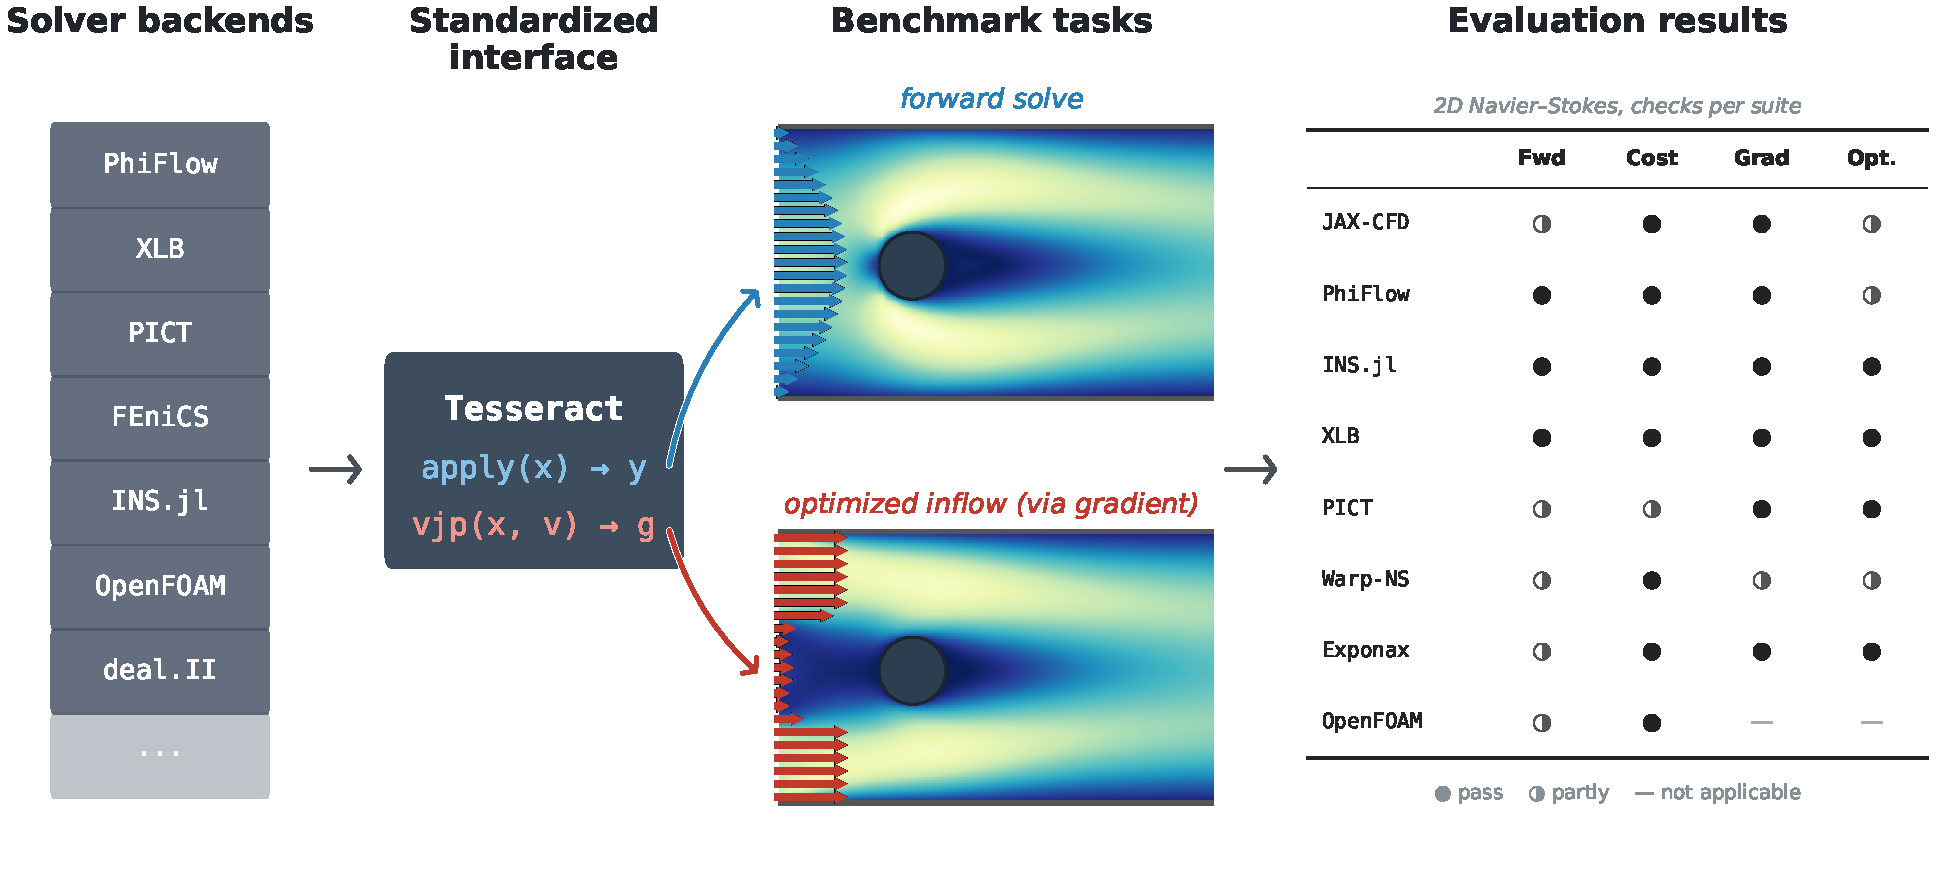
\includegraphics[width=\linewidth]{figures/visual_abstract.pdf}
  \caption{Overview of Mosaic. Diverse solvers are
    wrapped behind a uniform containerized interface, enabling cross-solver comparison on shared benchmark tasks involving different physical domains.}
  \label{fig:teaser}
\end{figure}

% ===========================================================================
\section{Introduction}
\label{sec:intro}

% Why it matters: differentiable solvers enable a broad family of techniques
Differentiable solvers enable topology
optimization~\cite{bendsoe2003topology}, aerodynamic shape
optimization~\cite{jameson1988aerodynamic}, optimal
control~\cite{bewley2001dns}, and solver-in-the-loop ML
training~\cite{kochkov2021machine, um2020sol} by backpropagating
through a numerical simulation's forward pass.
Differentiating through ODE integrators~\cite{chen2018neural,rackauckas2021universal}
and renderers~\cite{kato2020differentiable} is now routine, but PDE
solvers are more complex, less standardized, and their gradient
properties far less understood.

% The problem: opaque effort, hidden incompatibilities
A growing number of physics solvers advertise gradient support,
spanning multiple languages, AD frameworks, and numerical methods.
Yet it is hard to know in advance what reliable gradients from any of
them will cost. Solvers range from turnkey applications to
composable frameworks and low-level kernel toolkits, each demanding
different expertise and integration effort. Runtime and memory overhead,
gradient accuracy, and stability over long rollouts have not been
systematically measured. Solver-specific constraints therefore surface
only after a practitioner has committed to a particular solver: some
solvers support only periodic domains or lack the boundary types a task
needs, some become unstable over long rollouts, and some return gradients
that exhaust memory or silently lose accuracy in settings their own tests
do not cover.

Learned surrogates and physics foundation models offer an alternative
path, with limitations of their own (\cref{sec:related}). Meanwhile,
decades of engineering have produced solvers that practitioners
trust for forward simulation. What is missing is not the solvers
themselves, which exist in abundance, but a standardized way to
access, compare, and trust their gradients.

We introduce \textit{Mosaic}, an extensible benchmark suite that
provides a uniform interface to a diverse set of differentiable solvers
across multiple physical domains, with benchmark tasks that are designed
to systematically isolate issues with solver gradients. An initial set of
tasks focuses on standalone optimization
problems without learned components, where finite differences provide
ground truth and the solver's gradient mechanism is the only variable
under test. Mosaic enables researchers to evaluate which solver fits their problem,
build ML and optimization pipelines on top of the
uniform interface, and stress-test failure modes before
committing to a particular stack. Our contributions are:
%
\begin{enumerate}\itemsep2pt
  \item A \textbf{benchmark suite and containerized solver interface}
    spanning 14 solvers across four physical domains (heat transfer,
    structural mechanics, 2D and 3D Navier--Stokes;
    \cref{tab:domains}). Each solver is wrapped behind a uniform
    forward/gradient API regardless of language or AD strategy, so
    researchers can run and compare real solvers without
    solver-specific expertise.
  \item A \textbf{standardized evaluation protocol} measuring gradient
    accuracy, computational cost, Jacobian conditioning, setup
    compatibility, and end-to-end optimization convergence.
  \item \textbf{Empirical findings} showing that, on our tasks, all solvers
    that produce gradients reach comparable optima, and that solvers are ruled
    out instead by setup incompatibilities, instabilities over long
    rollouts, and the memory cost of their gradients.
  \item An \textbf{open-source release} of all solver interfaces, evaluation
    code, and templates, extensible to new solvers and domains, with
    CI-based re-evaluation infrastructure that keeps published results
    current as solvers improve.
\end{enumerate}

% ===========================================================================
\section{Background and related work}
\label{sec:related}

\paragraph{Adjoint methods and differentiable physics}
Adjoint methods for PDE-constrained optimization date back to
Lions~\cite{lions1971optimal}, and were brought to fluid design by
Pironneau~\cite{pironneau1974optimum} and
Jameson~\cite{jameson1988aerodynamic}, with discrete adjoint
formulations following in~\cite{giles2000introduction,nadarajah2000studies}.
Modern AD frameworks now differentiate solver code automatically:
JAX source transformation~\cite{bradbury2018jax}, PyTorch operator
overloading~\cite{paszke2019pytorch}, Julia source-to-source AD via
Zygote~\cite{innes2018don}, LLVM-IR-level AD via
Enzyme~\cite{moses2020enzyme}, NVIDIA
Warp kernel-level AD~\cite{macklin2024warp}, and tape-based discrete
adjoints in dolfin-adjoint and
firedrake-adjoint~\cite{farrell2013automated}.
Hand-derived adjoints are fast but tied to a fixed set of objectives,
requiring new derivations whenever the control variable or loss function
changes. Algorithmic AD removes this constraint at the price of higher
memory or computational cost, a tradeoff whose magnitude has remained
largely anecdotal. Mosaic measures this tradeoff empirically across solver families.

\paragraph{Learned surrogates and physics foundation models}
Neural operator surrogates~\cite{kovachki2023neural,li2021fourier,lu2021learning},
PINNs~\cite{raissi2019physics}, and physics foundation
models~\cite{pathak2022fourcastnet,bodnar2024aurora,price2024gencast,hao2024dpot,herde2024poseidon}
are complementary to differentiable solvers but introduce approximation
error, degrade outside the training distribution, require solver-generated
training data in the first place, and so far cover only a few well-studied
PDE families. Mosaic benchmarks the solver layer directly.

\paragraph{Existing benchmarks and evaluation efforts}
Several benchmarks evaluate PDE solvers or learned surrogates, but none
systematically measures gradient properties across solver backends.
APEBench~\cite{koehler2024apebench} benchmarks neural PDE emulators on
forward accuracy without evaluating solver gradients.
PDEBench~\cite{takamoto2022pdebench} provides datasets of PDE solutions
for surrogate training but includes no gradient evaluation.
NeuralFluid~\cite{fei2024neuralfluid} pairs a differentiable
Navier--Stokes solver with a benchmark of design and control tasks and
compares its forward and backward runtime against PhiFlow, yet
does not assess gradient accuracy, conditioning, or setup compatibility across backends.
List et al.~\cite{list2024differentiability} analyze gradient behavior in
unrolled training, focusing on convergence dynamics rather than
cross-solver comparison.
The PhiFlow benchmark~\cite{holl2024phiflow} compares AD backends within
a single framework, not across independent solver implementations.
preCICE~\cite{bungartz2016precice} standardizes solver coupling but
provides no gradient interface.

The closest analogue in design philosophy is OpenAI Gym~\cite{brockman2016openai}, which standardized access to RL
environments behind a uniform \texttt{step}/\texttt{reset} interface.
Gym ships no RL algorithms, yet the standardized interface enabled a
wealth of downstream research by lowering the barrier to entry.
Mosaic follows the same model for differentiable solvers: solver
backends are simulators behind a standardized gradient interface, and
the benchmark ships no ML components itself but provides the
infrastructure that researchers and practitioners can build on.
\Cref{sec:sil} reports one such study.

% ===========================================================================
\section{The Mosaic benchmark suite}
\label{sec:mosaic}

Mosaic organizes evaluation around three concepts. A \emph{physical
setup} is a concrete problem instance: a specific geometry, boundary
conditions, and operating regime within a physical domain (e.g.,
incompressible fluids). A \emph{benchmark task} is a fixed optimization
problem on a specific setup: a control variable, an objective, and a
reference solution. A \emph{solver backend} is
the software that evaluates the forward map and (optionally) its
gradient. Every solver that supports a
task's physical domain can be compared on it.

\subsection{Physical domains and benchmark tasks}
\label{sec:domains}

Benchmark tasks are representative optimization problems (inflow
optimization, topology optimization, inverse problems) that require
gradients for efficient solution, are supported by multiple backends
for cross-solver comparison, and contain no learned components so solver
gradients can be validated in isolation. Tasks are intentionally simpler
than state-of-the-art problems, as complexity in the physics could
confound the gradient properties we aim to isolate. This allows us to
attribute failures to the solver's gradient computation rather than to an
ill-posed optimization problem. The heat domain (H) additionally serves
as a negative control. Its forward problem is smooth and elliptic, so
any gradient failure on H is attributable to an AD bug rather than to
chaotic dynamics.
\Cref{tab:domains,fig:domains} summarize the four domains, and
\cref{app:effort} gives their full specifications.

\begin{table}[t]
  \centering\small
  \caption{Physical domains and optimization tasks. The backend count
    includes forward-only references; per-solver details are in
    \cref{tab:solvers}.}
  \label{tab:domains}
  \begin{tabularx}{\linewidth}{c>{\hsize=0.95\hsize}X>{\hsize=1.05\hsize}Xlll}
    \toprule
    \textbf{ID} & \textbf{Domain}
      & \multicolumn{2}{c}{\textbf{Optimization task}} & \textbf{Backends} \\
    \cmidrule(lr){3-4}
    & & \textit{Task} & \textit{Control dim.} & \\
    \midrule
    H & Heat transfer (slab) & Conductivity inversion
      & 128 & 5 \\
    & \multicolumn{2}{l}{\textit{%
      Negative control: smooth physics isolates AD bugs}} & & \\[5pt]
    S & Structural mech.\ (cantilever) & Compliance minimization (SIMP)
      & 256 & 6 \\
    & \multicolumn{2}{l}{\textit{%
      Well-studied topology optimization with known optimum}} & & \\[5pt]
    F2 & Incompr.\ fluids (2D cylinder) & Inflow optimization for drag min.
      & 41 & 8 \\
    & \multicolumn{2}{l}{\textit{%
      Anchor domain: standard channel benchmark, plus periodic checks}} & & \\[5pt]
    F3 & 3D Navier--Stokes (periodic) & Initial condition recovery
      & 12\,288 & 8 \\
    & \multicolumn{2}{l}{\textit{%
      Scale test: large states and long rollouts in a periodic box}} & & \\
    \bottomrule
  \end{tabularx}
\end{table}

\begin{figure}[t]
  \centering
  \begin{subfigure}[t]{0.48\linewidth}
    \centering
    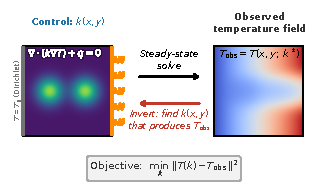
\includegraphics[width=0.95\linewidth]{figures/domain4_heat.pdf}
    \caption{\textbf{H}\,: Conductivity inversion in steady heat conduction.}
    \label{fig:domain_h}
  \end{subfigure}\hfill
  \begin{subfigure}[t]{0.48\linewidth}
    \centering
    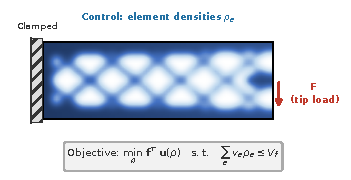
\includegraphics[width=0.95\linewidth]{figures/domain3_structures.pdf}
    \caption{\textbf{S}\,: Compliance minimization of a cantilever (SIMP).}
    \label{fig:domain_s}
  \end{subfigure}\\[0.2em]
  \begin{subfigure}[t]{0.48\linewidth}
    \centering
    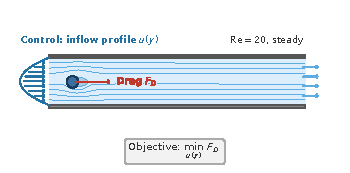
\includegraphics[width=0.95\linewidth]{figures/domain1_2d_fluids.pdf}
    \caption{\textbf{F2}\,: Inflow optimization for a 2D cylinder.}
    \label{fig:domain_f2}
  \end{subfigure}\hfill
  \begin{subfigure}[t]{0.48\linewidth}
    \centering
    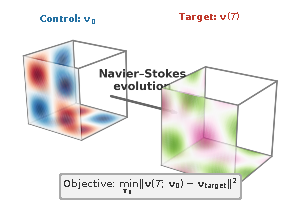
\includegraphics[width=.85\linewidth]{figures/domain2a_3d_ic_recovery.pdf}
    \caption{\textbf{F3}\,: Initial condition (IC) recovery in a 3D periodic box.}
    \label{fig:domain_f3}
  \end{subfigure}
  \caption{Benchmark tasks across the four physical domains in Mosaic.
    Each panel shows the control variable, the physical process,
    and the optimization objective.}
  \label{fig:domains}
\end{figure}

\subsection{Design principles}
\label{sec:scope}

Mosaic consists of three artifacts: a containerized solver interface,
an evaluation protocol, and a library of benchmark task templates.
Containerization is handled by Tesseract~\cite{haefner2025tesseract},
an existing open-source runtime for packaging scientific codes. Mosaic
contributes the evaluation methodology, benchmark tasks, and empirical
results on top of it. The four domains and 14 solver backends described
in this paper are its initial instantiation.

\paragraph{Solver interface and extensibility}
Each solver is wrapped as a containerized component exposing two entrypoints,
\texttt{apply(inputs)\,$\rightarrow$\,outputs} and
\texttt{vector\_jacobian\_product(inputs, cotangents)\,$\rightarrow$\,vjp}.
The container isolates all dependencies (language, libraries, GPU
runtime), so any of the 14 backends can be swapped by changing a single
configuration string.
Forward-only solvers
(OpenFOAM, deal.II) implement \texttt{apply} only and serve as forward
reference baselines.
Because solver APIs differ too widely for a single generic wrapper, each
benchmark task defines a \emph{task-specific interface schema} (inputs,
outputs, shapes, and units) that multiple solvers implement. To add a
backend, a contributor packages the solver as a Tesseract that implements
the task schema, and the evaluation suite re-runs automatically on every
proposed change.

Each benchmark task acts as a validated template with known-good settings,
so users can modify the physical setup (geometry, Reynolds number, boundary conditions) while
inheriting the evaluation protocol and finite-difference reference.
\Cref{app:software} describes how to contribute, and \cref{app:cost}
quantifies the overhead of containerization.

\subsection{Evaluation protocol}
\label{sec:protocol}

All metrics are computed uniformly across solvers. The protocol is
solver-agnostic: it operates on the containerized interface (forward and
VJP) and never inspects solver internals.

\begin{description}\itemsep2pt
  \item[Setup compatibility.] For each solver--task pair, we record
    whether the solver produces a gradient, fails numerically, or is
    structurally unable to represent the task (\cref{sec:optimization}).
  \item[Forward accuracy.] We compare accuracy across resolutions against a reference
    (a cross-solver consensus, or a converged spectral run for F3 and
    Kolmogorov flow) and verify adherence to physical laws where applicable
    (e.g., solenoidal velocity). Where an analytical solution exists (F2),
    precision is additionally measured against it.
  \item[Gradient accuracy.] Central finite differences through each
    solver's own forward pass serve as the reference. We
    evaluate directional derivatives along $K$ random perturbation
    vectors ($K{=}6$--$20$) and report cosine similarity and relative
    error for all problems. Besides the channel, F2 includes periodic
    setups that provide two further checks. For the decaying Taylor--Green
    vortex, the closed-form solution gives exact gradients with respect to
    the initial field and $\nu$ (\cref{tab:gradchecks}). On forced
    Kolmogorov flow, a common testbed for learned flow
    correction~\cite{kochkov2021machine}, we check the gradient through 16
    chained calls, as in a training loop (\cref{app:kolmogorov}). For the
    two Navier--Stokes problems (F2, F3), we also compute the full
    Jacobian and inspect its singular value spectrum.
  \item[Performance.] We measure primal and VJP wall-clock time, their
    ratio, and peak GPU (device-wide) and host memory on each solver's intended
    hardware target across various problem sizes (grid resolutions or cell counts).
    The VJP time is the cost of one gradient from scratch, a forward plus an
    adjoint pass.
    All timings are medians of 3 trials (10 on the mesh domains) after one
    warmup call to pre-populate JIT caches and stabilize memory allocation.
  \item[Optimization convergence.] We run fixed optimizers with each
    solver's gradients on each benchmark task for a fixed iteration budget,
    and compare the convergence curves and final objectives across solvers.
    \Cref{app:recovery} lists the budgets and optimizer settings, and the
    pass thresholds behind the \textit{Conv.} column of \cref{tab:merged}.
\end{description}

\subsection{Included solver backends}
\label{sec:solvers}

The solver set (\cref{tab:solvers}) is chosen to maximize diversity
along three axes: \emph{AD strategy} (autodiff, tape-based discrete
adjoints, hand-derived/kernel adjoints), \emph{numerical method} (projection-based, lattice Boltzmann,
finite-volume, spectral, finite elements with both direct and iterative
linear solvers), and \emph{solver abstraction level}.
These range from self-contained \emph{applications} (OpenFOAM),
through \emph{frameworks} that handle discretization and AD (FEniCS,
PhiFlow, JAX-CFD), to \emph{kernel toolkits} (NVIDIA Warp) where the
Mosaic wrapper \emph{is} the solver. Abstraction level determines
available gradient strategies and per-setup effort.

\begin{table}[t]
  \centering\small
  \caption{Solver backends included in the current release.
    Domain IDs match \cref{tab:domains}.}
  \label{tab:solvers}
  {\setlength{\tabcolsep}{4pt}
  \begin{tabular}{@{}llllll c@{}}
    \toprule
    \textbf{Solver} & \textbf{\shortstack[l]{Language /\\AD framework}}
      & \textbf{Strategy}
      & \textbf{\shortstack[l]{Discret-\\ization}} & \textbf{Numerics}
      & \textbf{GPU} & \textbf{Domains} \\
    \midrule
    JAX-CFD~\cite{kochkov2021machine}
      & Py/JAX & AD & FD & Projection, RK4 & $\checkmark$ & F2, F3 \\
    PhiFlow~\cite{holl2024phiflow}
      & Py/JAX & AD-S & FD & RK4/semi-Lagr. & $\checkmark$ & F2, F3 \\
    INS.jl~\cite{agdestein2024ins}
      & Julia/Zygote & AD & FV & Projection, RK4 & $\checkmark$ & F2, F3 \\
    XLB~\cite{ataei2024xlb}
      & Py/JAX & AD-C & LBM & BGK, float64 & $\checkmark$ & F2, F3 \\
    PICT~\cite{franz2025pict}
      & Py/PyTorch & AD-S & FV & PISO, BDF1 & $\checkmark$ & F2, F3 \\
    Warp-NS~\cite{macklin2024warp}
      & Py/Warp & AD/AD-S & FD & Projection, Euler & $\checkmark$ & F2, F3 \\
    Exponax~\cite{koehler2024apebench}
      & Py/JAX & AD & Spectral & ETDRK2 & $\checkmark$ & F2, F3 \\
%   FEniCS-NS~\cite{farrell2013automated}
%     & Py & Sym.+Auto & FE & IPCS, Crank-Nicolson & & F3 \\
    OpenFOAM~\cite{weller1998tensorial}
      & C++ & $-$ & FV & PISO/PIMPLE, Euler & & F2, F3 \\
    \midrule\midrule
    FEniCS~\cite{farrell2013automated}
      & Py & VA & FE & Direct (MUMPS) & & H, S \\
    Firedrake~\cite{rathgeber2016firedrake}
      & Py & VA & FE & Direct (MUMPS) & & H, S \\
    JAX-FEM~\cite{xue2023jaxfem}
      & Py/JAX & AD-S & FE & BiCGSTAB+Jacobi & $\checkmark$ & H, S \\
    TopOpt.jl~\cite{huang2021topoptjl}
      & Julia & HA & FE & Direct (CHOLMOD) & & S \\
    torch-fem~\cite{meyer2024torchfem}
      & Py/PyTorch & AD-S & FE & CG+Jacobi & $\checkmark$ & H, S \\
    deal.II~\cite{bangerth2007dealii,arndt2023dealii}
      & C++ & $-$ & FE & Direct (S), CG+AMG (H) & & H, S \\
    \bottomrule
  \end{tabular}}
  \par\vspace{4pt}
  \begin{minipage}{\linewidth}\footnotesize\raggedright
    \textit{Strategy:}
    AD\,=\,reverse-mode AD storing every step;
    AD-C\,=\,AD with checkpointing;
    AD-S\,=\,AD with adjoint linear solves;
    VA\,=\,variational adjoint (pyadjoint);
    HA\,=\,hand-derived adjoint;
    $-$\,=\,forward-only;
    a slash separates periodic box and channel.
    \textit{Discr.:}
    FD\,=\,finite differences;
    FV\,=\,finite volume;
    FE\,=\,finite elements;
    LBM\,=\,lattice Boltzmann method.
    \textit{Numerics:}
    PISO\,=\,pressure-implicit with splitting of operators;
    PIMPLE\,=\,merged PISO-SIMPLE;
    BDF1\,=\,1st-order backward differentiation;
    ETDRK\,=\,exponential time-differencing Runge--Kutta;
    BGK\,=\,Bhatnagar--Gross--Krook.
  \end{minipage}
\end{table}

\paragraph{Inclusion and exclusion criteria}
A differentiable solver is included if it provides a reverse-mode VJP for
arbitrary cotangents at the cost of a few forward solves, independent of
the number of inputs. This rules out, for example, solvers that offer only
forward-mode AD, whose gradient costs one pass per input dimension, as
finite differences do. Established forward-only solvers are included as
reference baselines for forward accuracy. Excluded solvers and reasons are
documented in \cref{app:solvers}.

% ===========================================================================
\section{Experiments}
\label{sec:experiments}

The following experiments check that Mosaic's evaluation protocol
distinguishes solvers in ways that matter in practice, and they provide an
initial empirical characterization to guide solver selection.
All experiments ran on an Azure \texttt{Standard\_NC24ads\_A100\_v4} instance
(one NVIDIA A100 80\,GB PCIe, 24 vCPUs of an AMD EPYC 7V13).
Results reflect the solver configurations of the pinned
release, and reproduction instructions are in \cref{app:software}.

\subsection{Benchmark summary and implementation effort}
\label{sec:baselines}

\Cref{tab:merged} summarizes benchmark results and implementation
effort across all solvers, and the subsections below discuss each metric.
Physical-accuracy validation is in \cref{app:physical_accuracy}, and the
reasons for setup incompatibilities are in \cref{app:exclusions}.

Implementation effort varies substantially among differentiable solvers.
We report bespoke lines of code (LOC) as a coarse proxy for integration
complexity, an imperfect metric but one that captures order-of-magnitude
differences reproducibly (\cref{app:effort}).
AD framework support does not guarantee turnkey gradients. PhiFlow, JAX-CFD,
and Exponax need at most 20 lines of gradient code, whereas INS.jl, PICT, and
XLB, which also differentiate through an AD framework, need 91 to 228.
The live version of Mosaic also records every departure from each solver's
default usage, together with how it works, whether it is required, and the
evidence for it, as guidance for practitioners integrating that solver.

\begin{table}
  \centering\footnotesize
  \setlength{\tabcolsep}{2.5pt}
  \caption{Benchmark results, gradient support, and integration effort per solver.
    Wall-clock times are medians of 3 (F2, F3) or 10 (S, H) timed trials
    after 1 warmup. Full specifications in \cref{app:effort}; initial conditions in
    \cref{app:ics}. Legend below table.}
  \label{tab:merged}
  \vspace{2pt}
  \begin{tabular}{@{}l r r c c c c | ccc | r r r@{}}
    \toprule
    \textbf{Solver}
      & \multicolumn{2}{c}{\textbf{Wall time}}
      & \multicolumn{3}{c}{\textbf{Error}}
      & \textbf{Conv.}
      & \multicolumn{3}{c|}{\textbf{Grad.\ support}}
      & \multicolumn{3}{c@{}}{\textbf{Integ.\ effort}} \\
    \cmidrule(lr){2-3}\cmidrule(lr){4-6}\cmidrule(lr){8-10}\cmidrule(lr){11-13}
    & \textit{Fwd} & \textit{VJP} & \textit{Ref.} & \textit{An.} & \textit{FD} &
      & \multicolumn{3}{c|}{\textit{input variables}}
      & \textit{IO} & \textit{Num.} & \textit{Conf.} \\
    \midrule
    \multicolumn{7}{@{}l}{\textit{Navier--Stokes grid (F2), wall time in ms}}
      & \textit{$v_0$} & \textit{$\nu$} & \textit{inflow} & & & \\
    \cmidrule(lr){8-10}
      Exponax~\cite{koehler2024apebench} & 26 & 46 & \textbf{3.3e-3} & \textbf{2.5e-6} & \textbf{4.1e-6} & $\bot$ & $\bullet$ & $\bullet$ & $\bot$ & 41 & 194 & \textbf{0} \\
      INS.jl~\cite{agdestein2024ins} & 160$^\dagger$ & 740 & 3.7e-3 & 2.4e-3 & 1.6e-5 & $\checkmark$ & $\bullet$ & $\bullet$ & $\bullet$ & 143 & 736 & 111 \\
      JAX-CFD~\cite{kochkov2021machine} & 20 & 40 & 3.7e-3 & 2.4e-3 & 7.1e-6 & $\bot$ & $\bullet$ & $\bullet$ & $\bot$ & 9 & 166 & \textbf{0} \\
      PhiFlow~\cite{holl2024phiflow} & 280 & 1500 & 3.7e-3 & 2.4e-3 & 1.0e-5 & $\checkmark$ & $\circ$ & $\circ$ & $\circ$ & 28 & 368 & \textbf{0} \\
      PICT~\cite{franz2025pict} & 1700 & 3900 & \textbf{3.3e-3} & 4.6e-3 & 4.6e-5 & $\checkmark$ & $\circ$ & $\circ$ & $\circ$ & 53 & 452 & 400 \\
      Warp-NS~\cite{macklin2024warp} & 83 & 320 & 3.6e-3 & 6.0e-4 & 3.7e-5 & $\checkmark$ & $\bullet$ & $\bullet$ & $\circ$ & \textbf{0} & 2405 & 14 \\
      XLB~\cite{ataei2024xlb} & \textbf{7.0} & \textbf{15} & 3.6e-3 & 6.1e-4 & 1.1e-5 & $\checkmark$ & $\bullet$ & $\bullet$ & $\bullet$ & 11 & 481 & 51 \\
      OpenFOAM~\cite{weller1998tensorial} & 1200 & $-$ & 3.6e-3 & 1.9e-3 & $-$ & $-$ & $-$ & $-$ & $-$ & 259 & \textbf{100} & 508 \\
    \midrule
    \multicolumn{7}{@{}l}{\textit{Navier--Stokes grid (F3), wall time in ms}}
      & \textit{$v_0$} &  &  & & & \\
    \cmidrule(lr){8-8}
      Exponax~\cite{koehler2024apebench} & 18 & 31 & \textbf{7.8e-4} & $-$ & 1.2e-4 & $\checkmark$ & $\bullet$ &  &  & 41 & 194 & \textbf{0} \\
      INS.jl~\cite{agdestein2024ins} & 140$^\dagger$ & 560 & 4.2e-2 & $-$ & 2.9e-5 & $\checkmark$ & $\bullet$ &  &  & 143 & 736 & 111 \\
      JAX-CFD~\cite{kochkov2021machine} & 19 & 37 & 4.2e-2 & $-$ & 2.0e-5 & $\checkmark$ & $\bullet$ &  &  & 9 & 166 & \textbf{0} \\
      PhiFlow~\cite{holl2024phiflow} & 160 & 370 & 4.0e-2 & $-$ & 1.8e-5 & $\checkmark$ & $\circ$ &  &  & 28 & 368 & \textbf{0} \\
      PICT~\cite{franz2025pict} & 550 & 1600 & 8.2e-3 & $-$ & 2.8e-5 & $\checkmark$ & $\circ$ &  &  & 53 & 452 & 400 \\
      Warp-NS~\cite{macklin2024warp} & 100 & 350 & 3.5e-3 & $-$ & 1.4e-5 & $\checkmark$ & $\bullet$ &  &  & \textbf{0} & 2405 & 14 \\
      XLB~\cite{ataei2024xlb} & \textbf{12} & \textbf{30} & 8.5e-3 & $-$ & \textbf{4.1e-6} & $\checkmark$ & $\bullet$ &  &  & 11 & 481 & 51 \\
      OpenFOAM~\cite{weller1998tensorial} & 3600 & $-$ & 2.2e-2 & $-$ & $-$ & $-$ & $-$ &  &  & 259 & \textbf{100} & 508 \\
    \midrule
    \multicolumn{7}{@{}l}{\textit{Structural mechanics (S), wall time in s}}
      & \textit{$\rho$} &  &  & & & \\
    \cmidrule(lr){8-8}
      FEniCS~\cite{farrell2013automated} & 4.2 & 8.7 & 0 & $-$ & 2.1e-5 & $\checkmark$ & $\circ$ &  &  & \textbf{0} & 334 & 63 \\
      Firedrake~\cite{rathgeber2016firedrake} & 1.8 & 3.9 & 0 & $-$ & 2.1e-5 & $\checkmark$ & $\circ$ &  &  & 39 & 263 & 137 \\
      JAX-FEM~\cite{xue2023jaxfem} & 1.5$^\dagger$ & 2.6$^\dagger$ & 0 & $-$ & 2.1e-5 & $\checkmark$ & $\circ$ &  &  & \textbf{0} & 203 & 109 \\
      TopOpt.jl~\cite{huang2021topoptjl} & 0.58$^\dagger$ & 0.62$^\dagger$ & 0 & $-$ & 2.1e-5 & $\checkmark$ & $\circ$ &  &  & 125 & 110 & \textbf{38} \\
      torch-fem~\cite{meyer2024torchfem} & \textbf{0.27} & \textbf{0.44} & 0 & $-$ & 2.1e-5 & $\checkmark$ & $\circ$ &  &  & \textbf{0} & \textbf{89} & 56 \\
      deal.II~\cite{bangerth2007dealii} & 2.4 & $-$ & 0 & $-$ & $-$ & $-$ & $-$ &  &  & 408 & 369 & 147 \\
    \midrule
    \multicolumn{7}{@{}l}{\textit{Heat transfer (H), wall time in s}}
      & \textit{$\rho$} & \textit{src} &  & & & \\
    \cmidrule(lr){8-9}
      FEniCS~\cite{farrell2013automated} & 1.0 & 2.3 & 6.1e-8 & $-$ & 1.8e-5 & $\checkmark$ & $\circ$ & $\circ$ &  & \textbf{0} & 507 & \textbf{61} \\
      Firedrake~\cite{rathgeber2016firedrake} & 0.37 & 0.74 & 6.1e-8 & $-$ & 1.8e-5 & $\checkmark$ & $\circ$ & $\circ$ &  & \textbf{0} & 305 & 102 \\
      JAX-FEM~\cite{xue2023jaxfem} & 0.38 & 0.77 & 6.1e-8 & $-$ & 1.8e-5 & $\checkmark$ & $\circ$ & $\circ$ &  & \textbf{0} & 275 & 100 \\
      torch-fem~\cite{meyer2024torchfem} & \textbf{0.14} & \textbf{0.20} & 6.1e-8 & $-$ & 1.8e-5 & $\checkmark$ & $\circ$ & $\circ$ &  & \textbf{0} & \textbf{220} & 70 \\
      deal.II~\cite{bangerth2007dealii} & 1.5 & $-$ & 6.1e-8 & $-$ & $-$ & $-$ & $-$ & $-$ &  & 401 & 284 & 77 \\
    \bottomrule
  \end{tabular}
  \par\vspace{2pt}
  \begin{minipage}{\linewidth}\scriptsize\raggedright
    \textit{Wall time} at $N=64$ (F2), $N=32$ (F3),
    $n_x=128$ (S), and $n_x=256$ (H);
    $^\dagger$\,=\,the trials vary by more than 15\% (\cref{tab:app:variance}).
    \textit{Error} (relative): Ref.\,=\,vs.\ reference at $\nu=0.01$ (F2: solver consensus,
    multimode IC; F3: Exponax at $N=64$), or the largest over the density sweep vs.\ the solver
    consensus (S, H), where the solvers agree to float32 round-off; An.\,=\,vs.\ analytical Taylor--Green solution at $\nu=0.01$;
    FD\,=\,vs.\ central finite differences (median over directions, best~$\varepsilon$).
    \textit{Conv.}\ (F2 drag, F3 L-BFGS+proj IC recovery, S topology opt., H conductivity recovery):
    $\checkmark$\,=\,passes the checks of \cref{app:recovery}; $\triangle$\,=\,flagged; $\times$\,=\,failed.
    \textit{Grad.\ support}: $\bullet$\,=\,AD through the solver; $\circ$\,=\,adjoint or
    hand-written VJP for at least part of it; $\times$\,=\,incorrect; $?$\,=\,not obtained;
    $\bot$\,=\,excluded (\cref{app:exclusions}); $-$\,=\,not applicable.
    Inflow support is shown only by a converged drag optimization.
    \textit{Integ.\ effort} (bespoke LOC): IO\,=\,input/output marshalling;
    Num.\,=\,numerics \& gradient code; Conf.\,=\,solver configuration.
  \end{minipage}
\end{table}


\subsection{Gradient quality}
\label{sec:quality}

We compare each solver's gradients against central finite differences at a
solver-specific optimal perturbation size~$\varepsilon$ and, on the periodic
F2 setup, against exact Taylor--Green gradients (\cref{tab:gradchecks}).

\begin{table}[t]
  \centering\small
  \caption{Gradient checks on F2. FD: relative error of the initial-condition VJP against
    central finite differences (median over directions at the best~$\varepsilon$).
    Analytic: relative error of the initial-condition gradient against the exact Taylor--Green
    gradient; $\mathrm{d}J/\mathrm{d}\nu$: relative error of the viscosity gradient against
    the exact one; both at $\nu=0.01$.}
  \label{tab:gradchecks}
  \begin{tabular}{@{}l c c c@{}}
    \toprule
    \textbf{Solver} & \textbf{FD} & \textbf{Analytic} & $\mathrm{d}J/\mathrm{d}\nu$ \\
    \midrule
      Exponax & \textbf{4.1e-6} & \textbf{1.3e-5} & \textbf{8.9e-6} \\
      INS.jl & 1.6e-5 & 1.9e-2 & 2.2e-2 \\
      JAX-CFD & 7.1e-6 & 1.9e-2 & 2.2e-2 \\
      PhiFlow & 1.0e-5 & 1.9e-2 & 2.2e-2 \\
      PICT & 4.6e-5 & 8.4e-3 & 4.3e-2 \\
      Warp-NS & 3.7e-5 & 4.9e-3 & 5.5e-3 \\
      XLB & 1.1e-5 & 1.9e-4 & 1.8e-3 \\
    \bottomrule
  \end{tabular}
\end{table}


All differentiable solvers reach cosine similarity $>0.999$ against finite
differences, consistent with correct AD. The optimal $\varepsilon$ differs by
orders of magnitude across solvers and domains, so a fixed step size can make
a correct gradient look wrong (\cref{fig:app:fdcheck}).

For the grid-based solvers, the forward discretization limits gradient
accuracy on the Taylor--Green checks. Every solver's error is larger against the
exact gradients than against finite differences, by three orders of magnitude
for the staggered-grid solvers, because the exact gradient also exposes the
discretization error that an optimizer sees. For these solvers, a more accurate
gradient would first require a finer discretization.

The three shapes of the F3 Jacobian spectra (\cref{fig:conditioning}) mostly
reflect how each solver treats initial perturbations that are not
divergence-free, which incompressible flow
forbids~\citep{guermond2006overview,bhatia2013helmholtz}. Solvers that project
them out exactly have singular values at round-off, so their condition numbers
measure round-off rather than the flow (\cref{app:gradient}). The spectra did
not indicate which solvers stay stable over long rollouts, since each shape
occurs both among solvers that stay stable and among those that return
non-finite gradients (\cref{sec:scaling}).

\begin{figure}[t]
  \centering
  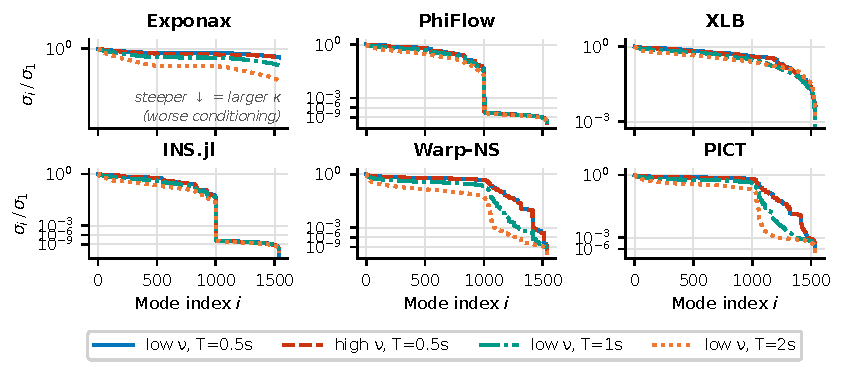
\includegraphics[width=\linewidth]{figures/jacobian_svd_comparison.pdf}
  \caption{Normalized Jacobian singular value spectra ($\sigma_i / \sigma_1$) on F3 ($N=8$) after $T=0.5$, 1, and 2 time units (10, 20, and 40 steps) at $\nu=10^{-3}$, and after $T=0.5$ at $\nu=10^{-2}$.
    Exponax and XLB keep a nearly flat spectrum at every rollout length. JAX-CFD, INS.jl, and PhiFlow drop to round-off after about two thirds of the modes, and the spectra of PICT and Warp-NS steepen as the rollout grows.}
  \label{fig:conditioning}
\end{figure}

\subsection{Computational cost and scaling}
\label{sec:scaling}

\begin{figure}[t]
  \centering
  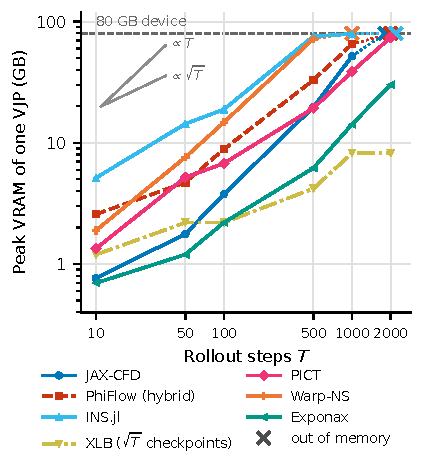
\includegraphics[width=0.755\linewidth]{figures/memory_rollout.pdf}
  \caption{Peak GPU memory of one VJP against rollout steps on F3
    ($N=48$), by differentiation strategy (line style).}
  \label{fig:memory_rollout}
\end{figure}

Absolute solver cost varies by orders of magnitude on the same problem
(\cref{tab:merged}; scaling curves in \cref{app:cost}), even between GPU
solvers that handle the same channel. XLB's explicit lattice Boltzmann
updates need no linear solve, whereas PICT's linear solves are bound by
device synchronization, and its F2 forward solve takes more than 200 times as
long.

Memory use depends on the differentiation strategy. Reverse-mode AD through a
time loop stores one state of size~$S$ for each of its $T$ steps, and hence
needs $O(T\cdot S)$ memory. Checkpointing, used here only by XLB, reduces this
to $O(\sqrt{T}\cdot S)$, and steady adjoints need only $O(S)$.
Unrolling $K$ inner solver iterations multiplies both the stored trajectory
and the cost of the reverse sweep by~$K$. By the implicit function theorem, a
solve-level adjoint instead needs only the converged state and one solve with
the transposed operator, which is why several solvers combine AD with adjoint
solves (AD-S in \cref{tab:solvers}). The F3 measurements follow these
scalings (\cref{fig:memory_rollout}), and without checkpointing, the stored
trajectory limits a $48^3$ rollout to a few thousand steps even with 80\,GB. Memory is not always the
first limit, however. On a longer F3 sweep, PhiFlow, Warp-NS, and XLB return
non-finite gradients after a few hundred steps, long before the other solvers
run out of memory (\cref{fig:horizon_sweep}). The steady mesh problems store
no trajectory and fail only at millions of elements (\cref{app:cost}).

Reverse-mode AD should cost a small constant multiple of the forward
pass~\cite{griewank2008evaluating}, and most VJPs here cost one to four
forward passes (\cref{tab:app:ratios}). This makes the ratio a cheap
diagnostic for integration problems. During development, ratios of up to
$1\,100$ exposed three integration bugs, all fixed in the reported results
(\cref{app:ratios}). INS.jl's ratio stays high at every grid size because
Zygote cannot differentiate the library's in-place time stepper, so its VJP
runs a slower non-mutating rollout instead.

\subsection{Optimization task performance}
\label{sec:optimization}

\begin{figure}[t]
  \centering
  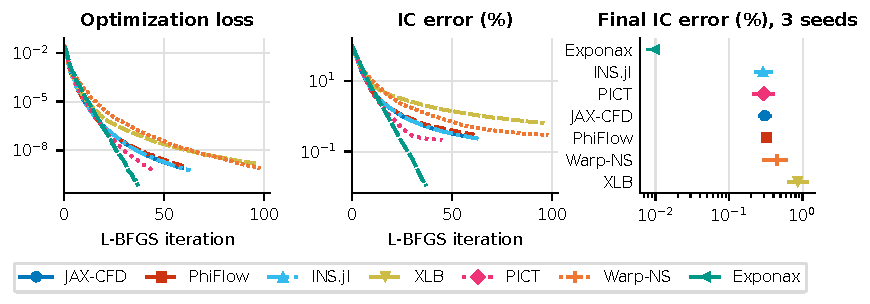
\includegraphics[width=\linewidth]{figures/recovery_main.pdf}
  \caption{F3 IC recovery for selected solvers and different optimizers. The IC
    error is the relative $\ell_2$ distance between the recovered and true initial
    states. Full version in \cref{fig:app:recovery}.}
  \label{fig:recovery_main}
\end{figure}

All solvers share the same hyperparameters and iteration budget per
task, so differences in convergence are attributable to the solver's
gradient alone. On every task, the solvers that can run it reach
comparable results (\cref{app:recovery}). They converge to the same optimum
on S and reduce drag by 46 to 48\% on F2. On H, every solver lowers the
misfit by about eight orders of magnitude, but the poorly conditioned
inversion leaves the recovered conductivity dependent on the optimizer's
path. Two solvers cannot run the F2 channel: Exponax represents only
periodic fields, and the JAX-CFD API cannot express the channel's inflow,
outflow, and obstacle.

On F3, the choice of optimizer matters more than the choice of solver
(\cref{fig:recovery_main}). L-BFGS recovers the initial state an order of
magnitude more accurately than Adam, in a fraction of the gradient
evaluations. Projecting the gradient onto divergence-free fields before each
L-BFGS update (L-BFGS+proj) improves the recovery on every solver, likely because it
keeps components that incompressible flow forbids out of the optimizer's
curvature model.

\subsection{Solver-in-the-loop training}
\label{sec:sil}

The benchmark checks gradients outside of any training loop. To test
whether these checks predict how a solver behaves inside one, we trained a
small periodic CNN to correct each solver's coarse ($64^2$) run of forced
Kolmogorov flow against the solver's own $256^2$ run, in three arms:
supervised one-interval pairs, a 16-interval rollout with the gradient
stopped at every solver call, and the same rollout differentiated through
the solver (SIL). Four solvers run the full study (JAX-CFD, INS.jl, XLB, and
Exponax), and \cref{app:sil} gives the setup and the reasons for excluding
the others.

The study exposed one gradient defect, PICT's adjoint tolerance, which
single-call checks miss and only the chained gradient check catches
(\cref{app:kolmogorov}). For the four solvers that run the study, whose
gradient errors are all below $2\times10^{-3}$, the test errors track forward
accuracy rather than gradient accuracy (\cref{tab:app:sil}). The two solvers
with the larger uncorrected error gain the most, and the other two still end
lower. Because each solver trains against its own reference and starts from
a different error, these gains are hard to compare across solvers.

Averaged over three seeds, supervised training reached the lowest test error
on every solver except Exponax, and SIL's average never beat the
stopped-gradient arm, although individual SIL seeds did. Earlier work found
training through the solver to outperform supervised
training~\cite{um2020sol} and, by a smaller margin, the stopped-gradient
rollout, also on Kolmogorov flow~\cite{list2024differentiability}. Our
corrector has about 2\,600 parameters and trains for 256 updates without a
curriculum or per-arm tuning, so this is not a fair test of that advantage.
Within this setup, the solvers differed under SIL training only in cost.

% ===========================================================================
\section{Discussion and conclusion}
\label{sec:conclusion}

Gradient accuracy, computational cost, memory, stability, and setup
compatibility vary widely across solvers. Some of these properties
determine whether a solver can serve a workflow at all, and others only how fast it does so. Based on our
benchmark tasks, we highlight five practitioner-facing observations.

\paragraph{Gradient quality is often good enough}
On every task where they can run, all solvers that produce gradients
reach comparable optima despite order-of-magnitude differences in
gradient accuracy. More complex tasks may make gradient quality limiting,
but these benchmarks suggest that optimization and training are often
robust to it. Solvers failed instead because they could not express the
task, turned unstable over long rollouts, or ran out of memory.

\paragraph{Rollout length is the critical scaling parameter}
For unrolled training and long-horizon control, two limits on rollout
length can make a solver unusable. Without checkpointing, memory limits most
F3 solvers at a few thousand steps on a $48^3$ grid, and three of seven solvers
return non-finite gradients after a few hundred steps (\cref{sec:scaling}). Both aspects should
be tested at the intended rollout length before committing to a solver.

\paragraph{On steady linear problems, pick the fastest (or friendliest) solver}
On problems H and S, all solvers produce equivalent
results regardless of AD strategy or numerical method, so the choice
reduces to forward speed at the intended size and integration effort.

\paragraph{Reverse-mode AD offers the best effort-to-capability tradeoff}
Hand-derived adjoints can be cheap, as TopOpt.jl's self-adjoint compliance
gradient costs about one forward solve (\cref{tab:merged}), but each new
control variable or objective requires new derivations. Reverse-mode AD
through modern frameworks produces gradients accurate enough for
optimization at a fraction of the implementation cost. At the sizes of
\cref{tab:merged}, AD gradients cost 1.4 to 5.3 times the forward time.

\paragraph{Measure rather than predict}
Some properties can be anticipated from how a solver works: memory scales with the differentiation strategy, gradient
accuracy is bounded by the discretization, and Fourier methods are
restricted to periodic domains. Some properties that decided whether a
solver was usable here could not. Solvers of the same numerical family and
AD strategy ended up on both sides of the stability limit, their Jacobian
spectra did not anticipate it (\cref{sec:quality}), and gradient defects
and the largest cost outliers came primarily from how a solver was built or wrapped.
Practitioners should therefore test candidate solvers on their own task, for
example by adapting one of Mosaic's task templates (\cref{sec:scope}).

\paragraph{Limitations}
Our conclusions rest on three choices. The gradient reference is central
finite differences at the best perturbation size, corroborated by the exact
Taylor--Green gradients. Each solver runs as published, with every
departure from its default usage recorded, and expert tuning of
resolution, time step, or preconditioner could narrow the gaps we observe.
Standalone optimization tasks stand in for broader pipelines, which the
solver-in-the-loop study supports for one setup.

The scope is deliberately narrow. The tasks are easy (small grids, moderate
Reynolds numbers, short rollouts, steady linear mesh problems), and only
the solver-in-the-loop study includes learned components. Results should
not be extrapolated to harder problems, such as fully developed 3D
turbulence, long-horizon optimization, or nonlinear mechanics, or to other
hybrid pipelines without further validation. All timings come from a
single A100 machine, and rankings may shift on other hardware, especially for
float64 solvers such as XLB on consumer GPUs with low float64 throughput.

The numbers are a snapshot of pinned solver versions, and rankings will
change as solvers improve. Tracking such changes is part of the benchmark's
purpose, and its continuous re-evaluation keeps the published results
current. We therefore deliberately state our conclusions in terms of general
failure modes and solver properties, and expect them to hold beyond individual
ranking changes.

\paragraph{Future work}
Natural extensions include additional domains (multiphysics, compressible
flow), solver backends (Enzyme/LLVM-level AD), and hybrid physics-ML tasks.
The infrastructure is in place, and we invite community contributions.
